\chapter{Architecture \& Modules Integration}
\label{chapter5}

\section{Architecture}

\begin{figure}[!htbp]
\begin{center}
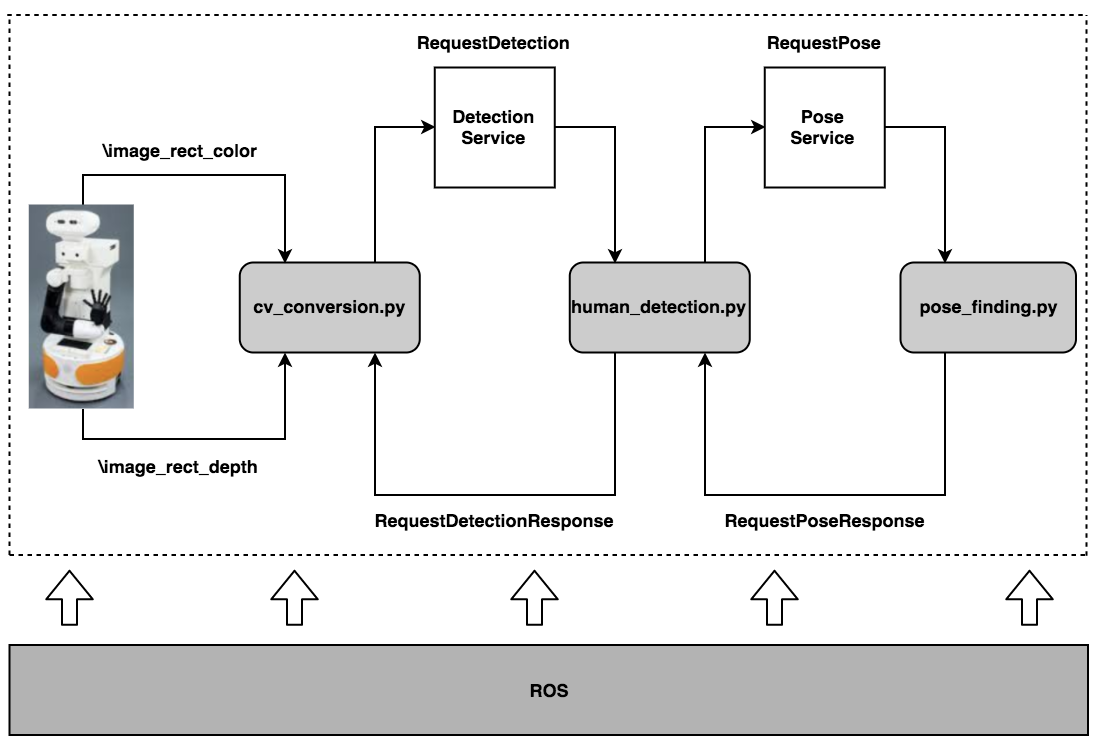
\includegraphics[width=\linewidth]{images/chapter6_architecture.png}
\end{center}
\caption{Project's architecture.}
\label{fig:architecture}
\end{figure}

The final solution has three main components to it:

\begin{enumerate}
	\item The conversion script that converts the \textbf{image\_rect\_color} into an OpenCV format.
    \item The detection script that detection people in the converted frame.
    \item The pose script that retrieves the detection's distance and finds its 3D pose.
\end{enumerate}

All of the components do sit on top of the ROS middleware presented in chapter 1 whose utilities including ROS services, standard messages and publish-subscribe type of communication were used. Moreover, it is essential to have a ROS master available for the package to work as this handles the topics and makes available the required topics such as the rectified coloured image and the rectified depth-image, where this, in this occasion were made available by TIAGo's bring-up and its ROS master export in the development machine. Lastly ROS services were used for module-intra-communication. Figure 5.1 gives an overview of how the communication happens between the various components.

\subsection{Communication Logic}

\subsection{Conversion}

The conversion module was implemented via a set of routines which are called by the main within the same file, which subscribes to the rectified colour and depth image, converts the former and sends a service request to the detection module, which will respond with a success of failure message (once the whole communication chain is resolved).

\subsection{Detection}

The detection module waits until the service request from the conversion script is received, and upon which it runs the feed-forward process, creates a detections message and passes this to the next module via a different service request, upon which is will remain idle until a response is sent back before taking any further action.

\subsection{3D Pose}

Lastly the pose module receives the request from the detection module, computes the per detection distance and retrieves its 3D pose in the map. Once done, a set of markers are published to RVIZ along with a custom poses message with the 3D pose for each detection, and a response notifying the success of failure of the process is sent back to the service caller.

\section{Modules Integration}

The original plan for the development consisted in having separate modules for each task that operate independently of each other, and that would have access to each others computations via the published topics. However, this had to be reconsidered when the pose and detection modules had to be integrated. In fact, given that the subscribed depth-image published by TIAGo's interface has a lower publishing rate then the coloured image, a synchronisation problem rose, where the wrong depth ROI\footnote{Region of Interest} was accessed because of the delay, which ultimately consisted in computing the wrong distance and therefore the wrong 3D pose.

\subsection{Time Synchroniser \& ROS Services}

\subsubsection{Time Synchroniser}

To solve the synchronisation issue an approximate time synchroniser was used. More precisely the \textbf{ApproximateTimeSynchronizer} routine made available by the message\_filters library allows the subscription to multiple topics whose callback function is called only when the timestamps differences are within a certain threshold. 

Therefore, two separate subscriptions called \textbf{rgb\_sub} and \textbf{depth\_sub} were made respectively to the RGB and the depth-image topics, in the \textbf{cv\_conversion.py} script, which consequently got chained together using the time synchronizer with a threshold error of at most 0.5 seconds, as shown below. Of course, the bigger the threshold, the greater the delay, hence a good empirical value had to be found. The synchronisation is then binded to a callback function called \textbf{processSubscriptions} using the \textbf{registerCallback} routine, also made available by the message\_filters library.

\begin{lstlisting}
import message_filters as mf
ats = mf.ApproximateTimeSynchronizer([rgb_sub, depth_sub], slop=0.5)
ats.registerCallback(processSubscriptions)
\end{lstlisting}

\subsubsection{ROS Services}

Two choices were available for the communication paradigm between the modules, either using standard publish-subscribe communication or an RPC based style via services. 

The original idea was to use the former type of communication, as it would allow a more flexible and modular usage of the package given that if a user only wants to use a specific function of it, only the required module/s need to be run. However, due to the RGB-depth synchronisation problem, and the fact that the subscriptions are both made in one place (the conversion script) and not in their relative module as originally planned (so rgb\_sub in the conversion module and depth\_sub in the pose module) the latter type of communication via ROS services was preferred for an easier message communication.

In fact, via a service mean, the collected ROS messages at subscription time can be passed forward to server nodes with simple \textbf{srv} files, rather then having to publish them all over again. Therefore two services were established, a detection one which has as a client the conversion module and as a server the detection one and which sends as input both the RGB and depth-image messages, as well as a pose service whose client is detection module and server the pose one which accepts both the synchronised depth-image and a Detections message introduced in Chapter3 as inputs.



